\chapter{Introdução}

Nas últimas décadas, presencia-se os acelerados avanços em ciência e tecnologia impulsionados por empresas dos mais diversos ramos e pelas constantes pesquisas nas universidades. 

Um dos avanços mais significativos é a Internet, com um grande impacto no desenvolvimento da economia global e na sociedade atual. Em duas décadas tem decorrido um grande crescimento na disponibilidade do acesso à rede. Em setembro de 2016, o número de usuários da rede mundial de computadores era de, aproximadamente, 3,75 bilhões, cerca de metade da população mundial e por volta de 92 vezes maior em relação ao ano 2000 \cite{MiniwattsMarketingGroup2016}.  Outro grande avanço se tem nos celulares, aos quais evoluíram tanto nos últimos anos que passaram de simples e grandes telefones sem fio à dispositivos menores, no entanto, com acesso a Internet, recursos avançados de áudio e vídeo e poder de processamento equiparável ao de computadores de mesa (\textit{desktops}) e/ou notebooks.

Em meio ao domínio da Internet, um novo paradigma surgiu no meio acadêmico e aos poucos ganha terreno nas grandes empresas. A sua proposta é levar a tecnologia a objetos do dia a dia, como condicionadores de ar, lâmpadas, fogões etc., e, assim, criar novas formas de interação além de funcionalidades inéditas, seguindo o exemplo dos \textit{smartphones}. 

Mencionada pela primeira vez, por Kevin Ashton, em 1999 \cite{Finep2015}, a Internet das Coisas ou IoT (em inglês, \textit{Internet of Things}) está cada vez mais próxima da realidade. Abrigará um variado ecossistema de dispositivos com capacidade de processamento, sensoriamento, conexão com demais dispositivos e, em muito casos, com a Internet, entre outros avanços. Estima-se que, em 2020, cerca de 24 bilhões de dispositivos IoT estejam conectados, implicando em cerca de quatro dispositivos por pessoa \cite{Meola2016}.   
Contudo, com o crescimento do número de itens computacionais, a quantidade de dados gerado por eles também cresce, mas de maneira exponencial \cite{Chiang2016}. A partir disso, o fluxo de dados na rede de internet se intensifica a ponto de comprometer o desempenho desta. Isso ocorre devido ao modelo atual de funcionamento da rede, ou seja, centralizado. Portanto, uma nova arquitetura se faz necessária para incorporar os dispositivos IoT à Internet tradicional. % já citado
Nesse contexto, a \textit{fog computing} ou computação de neblima, surge como potencial solução, com base na proposta de uma nova forma de organização de rede para complementar a atual. Isso é possível com base na aproximação de algumas funcionalidades centralizadas em servidores aos dispositivos que as utilizam \cite{Chiang2016}. Para tanto, um dispositivo de rede seria responsável por uma \textit{nuvem local}. Assim, os dispositivos IoT se comunicariam com esse equipamento e obteriam funcionalidades necessárias de maneira mais eficiente. A nuvem local se comunicaria diretamente com a nuvem convencional, transferindo apenas informações necessárias \cite{Syed2016}.

Os objetos inteligentes, ou \textit{smart objects}, com funcionalidades expandidas como comunicação, sensoriamento, processamento e atuação sobre o ambiente, promovem a interação entre o mundo físico (analógico) e o mundo digital \cite{Stojkoska2017}. Isso ocorre graças a sensores capazes de capturar grandezas como temperatura e luminosidade e, a partir disso, permite que aplicações tenham conhecimento do contexto do ambiente. Baseando-se nesses conceitos, algumas companhias vêm colocando no mercado novos produtos com características citadas. Como exemplo, é citável o Amazon Echo\textsuperscript{\textregistered}\footnote{https://www.amazon.com/Amazon-Echo-Bluetooth-Speaker-with-WiFi-Alexa/dp/B00X4WHP5E}, um dispositivo que opera com o serviço de assistente pessoal Alexa, e interage com pessoas em uma casa a partir de comando de voz. Outro produto destacável, é a \textit{smart lock} da empresa Nuki\textsuperscript{\textregistered}\footnote{https://nuki.io/en/shop/nuki-smart-lock/}, pelo qual é possível abrir e fechar a porta apenas com um toque no aplicativo móvel pelo \textit{smartphone} ou através de um \textit{smart watch}. Por outro lado, áreas como esportes também recebem atenção. O CARV\textsuperscript{\textregistered}\footnote{https://www.kickstarter.com/projects/333155164/carv-the-worlds-first-wearable-that-helps-you-ski}, um dispositivo vestível ou \textit{wearable}, ao qual propõe um calçado para praticantes de ski capaz de analisar em tempo real o modo de esquiar e fornecer informações detalhadas sobre.

Os \textit{smart objects} poderão, a partir da IoT, operar em conjunto e comporem os chamados \textit{smart environments}, ambientes nos quais a integração dos dispositivos agrega novas funcionalidades e formas de interação para aquele ambiente \cite{Asano2016}. Entre os ambientes inteligentes emergentes estão as \textit{smart grids}, às quais propõem a atualização do sistema elétrico atual a partir do uso da tecnologia. Uma das principais mudanças será o direcionamento do fluxo de energia e informações em dois sentidos. Como consequência, será possível consumir e fornecer energia para o sistema elétrico, bem como trocar informações sobre o estado da rede de eletricidade, o consumo entre outros avanços. Tudo isso será viável em virtude da capacidade de sensoriamento, troca de informações, controle e de tecnologia da informação e comunicação \cite{Cecilia2016}.  

Além das \textit{smart grids}, outro ambiente em expansão é a \textit{smart home}. Através dela, os moradores de uma casa podem interagir com um ambiente inteligente capaz de responder ao seus comportamentos e prover diversas funcionalidades \cite{DeSilva2012}. Isso se deve à presença de dispositivos dotados com tecnologias de sensoriamento, controle e comunicação. Além disso, a integração desse ambiente com a \textit{smart grid} pode propiciar um aumento na eficiência do consumo da casa, a partir do gerenciamento dos dispositivos conectados implicando, desse modo, menos gastos com eletricidade no final do mês (citar). %TODO: Citar

Os ambientes inteligentes podem abrigar outros menores. No caso das \textit{smart homes}, é possível subdividí-las em ambientes como a cozinha inteligente ou \textit{smart kitchen}. Nesse ambiente, usuário tem à disposição novas maneiras de interagir com os utensílios na preparação de alimentos, eletrodomésticos entre outros. A partir disso, surgem diversas oportunidades em termos de criação de produtos, como geladeiras, fogões, cafeteiras conectadas. Em relação às geladeiras inteligentes ou \textit{smart fridges}, por exemplo, viu-se um avanço nos últimos anos. Desde os anos 2000 vem-se pensando em como conectar refrigeradores à Internet, com a LG\textsuperscript{\textregistered}\footnote{http://www.lg.com} entre as primeiras companhias a implementar o conceito de dispositivos conectados à Internet. Em pesquisas recentes, propõe-se adicionar outros recursos como monitoramento dos produtos no interior e seus respectivos prazos de validades entre outros \cite{Hachani2016}. 

As interações das pessoas com os ambientes citados gerará uma grande quantidade de dados. Um aproveitamento eficiente desses dados pode ampliar as aplicações da IoT. Uma das diversas formas para colocar essa ideia em prática são os sistemas de recomendação. Com base nas preferências indicadas pelo usuário ou no seu comportamento, esses sistemas buscam selecionar e fornecer informações relevantes \cite{Filho2008}. Sistemas de recomendação são divididos em duas classes: filtragem colaborativa em que as recomendações são feitas com base na similaridade das preferências de usuários com os demais, isto é, em gostos de outros usuários em produtos, serviços etc., que o usuário não conhece, mas tem alta probabilidade de interesse. Outra categoria é a baseada em conteúdo, na qual os conteúdos apresentados ao usuário são baseados nas suas próprias preferências, ou seja, em itens semelhantes aos de interesse. Por fim, existe a abordagem mista, em que ambas as categorias citadas são mescladas, aproveitamento, desse modo, as melhores características de cada uma \cite{Thomas2016}.
Além disso, as aplicações de sistemas de recomendação são adotadas nos mais diversos campos, entre eles, plataformas de streaming de filmes e séries, sites de vendas online entre outros. Ainda assim, os sistemas de recomendação vêm recebendo novas propostas de uso como sistemas aptos a propor pontos de carga para condutores de carros elétricos \cite{Ferreira2011} e notícias personalizadas \cite{Yeung2010}. 

% TODO: Escrever sobre HCI

\section{Problemática}
% Explicação:
% A problemática deve enfatizar os desafios identificados na literatura, ou seja, durante a leitura dos artigos alguns desafios foram identificados nas áreas de pesquisa do trabalho (Internet das Coisas, Smart Things ou correlatos, Sistemas de Recomendação) e devem ser apresentados. A partir da dissertação sobre tais desafios se finaliza a seção com uma pergunta de pesquisa, geralmente iniciando pela palavra "Como".


Com o avanço da Internet das Coisas, a rede de internet necessitará de algumas adaptações para suportar o grande número de dispositivos conectados e alto volume de dados que serão transmitidos a todo momento. Além disso, como cada dispositivo estará vinculado à rede, ele estará, portanto, ao alcance de ciber criminosos. No entanto, a segurança em IoT não evoluiu suficientemente para garantir preservação desses dispositivos.

Em relação as geladeiras inteligentes, um dos problemas no monitoramento e registro de itens em uma geladeira é o modo com o qual é realizado. Muitas propostas fazem uso de dispositivos que operam por ondas eletromagnéticas. No entanto, os alimentos que contém água além de estruturas metálicas podem interferir no desempenho das leituras a depender da tecnologia utilizada \cite{Periyasamy2015} \cite{Qing2007}. Por outro lado, os métodos que utilizam processamento de imagem têm êxito em monitoramento de alimentos naturais como verduras e frutas \cite{Shweta2017}, mas não há propostas que englobe processamento de imagem para produtos embalados, como leite, enlatados entre outros na literatura.

Apesar do grande número de estudos a cerca da IoT, as tecnologias e aplicações propostas não têm dado devida atenção aos aspectos de usabilidade e experiência do usuário, focando mais no ponto de vista técnico \cite{Koreshoff2013}. É necessário portanto, incluir no projeto de aplicações o conceito de interface humano e tecnologia.

% Concluir com a pergunta de pesquisa
Desse modo, tem-se como pergunta de pesquisa: ``Como melhorar o modelo de geladeira comum que capture a interação com os usuários permitindo a estes experiências que facilitem o seu dia a dia na cozinha?''.

% V1: Como projetar uma geladeira inteligente com experiência única aos seus usuários e lhes proporcionar uma melhor qualidade de vida?
% V2: Como projetar uma geladeira inteligente que capture a interação com os usuários permitindo a estes experiências que facilitem o seu dia a dia na cozinha.
% V3: Como melhorar o modelo de geladeira atual que capture a interação com os usuários permitindo a estes experiências que facilitem o seu dia a dia na cozinha?.

\section{Objetivos}
Esta seção apresenta o objetivo geral e os objetivos específicos do trabalho.

\subsection{Geral}

% V1: Desenvolver uma geladeira capaz de monitorar os produtos contidos nela e prover recomendações de receitas com base nos padrões de consumo dos produtos.

% Desenvolver uma geladeira que facilite o dia a dia dos usuários a partir da análise das interações entre os mesmos.

Desenvolver um modelo de geladeira inteligente que facilite o dia a dia dos usuários a partir da análise das interações entre os mesmos.
    
% V4 Melhorar o modelo de geladeira inteligente para que facilite o dia a dia dos usuários a partir da análise das interações entre os mesmos.

\subsection{Específicos}


\begin{itemize} \parskip -1pt
	%\item Levantamento do estado da arte com relação a Internet das Coisas e Sistemas de Recomendação
	\item Elaborar e desenvolver um projeto de leitura e monitoramento dos produtos contidos na geladeira.
	\item Implementar um sistema de análise das interações e recomendação de serviços.
	\item Elaborar um cenário que permita a avaliação do modelo proposto.
	\item Avaliar e discutir os resultados obtidos a partir do sistema proposto.

%V1
% 	\item Levantar o estado da arte com relação a Internet das Coisas e Sistemas de Recomendação
% 	\item Propor um projeto de leitura e monitoramento dos produtos contidos na geladeira.
% 	\item Propor um sistema de análise das interações e recomendação de serviços.
% 	\item Elaborar um cenário que permita a avaliação do sistema proposto.
% 	\item Avaliar e discutir os resultados obtidos a partir do sistema proposto.

\end{itemize}

\section{Justificativa e Motivação}

A Internet tem evoluído nas últimas décadas e impactado na economia mundial e no dia a dia das pessoas. Nos seus primeiros anos de existência, tinha como principal função o uso militar e acadêmico, como foco em troca de informações \cite{Leiner2012}. Contudo, anos mais tarde foi aberta para uso da população em geral permitindo, desse modo, que pessoas comuns tivessem acesso a rede. Hoje, cerca de metade da população mundial usam a Internet frequentemente \cite{MiniwattsMarketingGroup2016}. 

No cenário atual, um novo grupo está sendo conectado na Internet: "as coisas". Cria-se um novo paradigma, a Internet das Coisas, onde a rede não será mais utilizada apenas da maneira tradicional, como em um computador de mesa ou \textit{smartphone} entre outros, mas por dispositivos que possuem acesso a redes e capacidades como sensoriamento, atuação e comunicação com outros dispositivos. Muitos dos dispositivos serão versões conectadas dos objetos presentes no dia a dia, como televisão, fogão, geladeira, lâmpada e porta. Todos esses equipamentos, operando em conjunto com a rede, criarão um ecossistema de objetos com funcionalidades inéditas. 

Com a IoT estima-se que até 2020, cerca de 24 bilhões de dispositivos estejam conectados \cite{Meola2016}, garantindo espaço para inovação em produtos e serviços. Além disso, espera-se que a Internet das Coisas se torne um grande atrativo para o mercado. Estima-se que em 2025 sejam gerados em torno de 13 trilhões de dólares (citar).

A sociedade se beneficia com o desenvolvimento da Internet das Coisas. As soluções geradas considerando esse conceito trarão novas formas de interação entre as pessoas e os objetos que as cercam no cotidiano. Ambientes como casa, indústria e sala de aula terão a disposição novas formas de interação com esses a partir da tecnologia. 

Tratando-se de uma casa inteligente, chamada também de \textit{smart home}, os moradores tem a disposição conforto e comodidade em virtude dos objetos conectados presentes nela, entre eles a geladeira. Presente em grande parte dos lares, o refrigerador tem um papel fundamental na vida dos moradores. Os alimentos contidos nela devem ser bem conservados para o consumo. No entanto, produtos são esquecidos no seu interior e, por vezes, passam do prazo de validade. Além disso, seria muito cômodo aos usuários, dessa geladeira, estando em um supermercado e soubessem quais itens estão faltando ou vencidos, evitando assim compras em demasia ou modéstia. Apesar da facilidade na visita ao supermercado com uma lista em tempo real dos produtos necessários, seria ainda mais cômodo se o refrigerador, automaticamente realiza-se compras de itens essenciais como leite ou carne e o supermercado entregasse as compras em casa. Ainda que tais funcionalidades não sejam comuns, existem propostas de geladeiras inteligentes que as implementam. Contudo, não há abordagens em que se leve em conta os interesses do usuários como preferências em certos alimentos, horários em que o consumo é mais comum entre outros. Por isso, acredite-se que entender o comportamento do usuário com IoT pode melhorar o dia a dia deste.

Portanto, este trabalho trará como contribuição a melhora do modelo atual de geladeira inteligente que além das funcionalidades citadas, leve em conta os interesses e padrões de consumo de seus usuários.


% V1: ...como contribuição a proposição e implementação de uma geladeira inteligente que além das funcionalidades citadas, leve em conta os interesses e padrões de consumo de seus usuários. 



\section{Procedimentos metodológicos}

% O que é metodologia
O método é a ordem que se deve impor aos diferentes procedimentos necessários para atingir um certo objetivo \cite{Cervo2007}. Por meio destes procedimentos, a pesquisa caracteriza-se como uma atividade voltada para a investigação de problemas teóricos ou práticos \cite{Matias-Pereira2012}.

% Tipo de pesquisa
Este trabalho pode ser caracterizado, quanto à sua finalidade, como uma pesquisa aplicada, visto que, conforme \citeonline{Matias-Pereira2012}, ``os conhecimentos adquiridos são utilizados para aplicação prática e voltados para a solução de problemas concretos da vida moderna''. Quanto ao objeto, o projeto é descrito como uma pesquisa bibliográfica, já que é necessária para o levantamento do estado da arte do tema, fundamentação teórica e definição da contribuição do trabalho \cite{Matias-Pereira2012}. De acordo com a modalidade, a pesquisa se identifica como uma pesquisa tecnológica, onde será criado um artefato tecnológico, sendo este um protótipo de geladeira capaz de reconhecer as interações do usuário, realizar compras automáticas além de recomendações de outros produtos e receitas com base nas preferências do usuário. 

A metodologia de desenvolvimento deste trabalho é dividida em 8 etapas, das quais, a ordem cronológica é apresentado na \reffig{cap1_metodologia-etapas}.

\begin{figure}[hb]
    
    \caption{Fluxo das Etapas do Trabalho}
    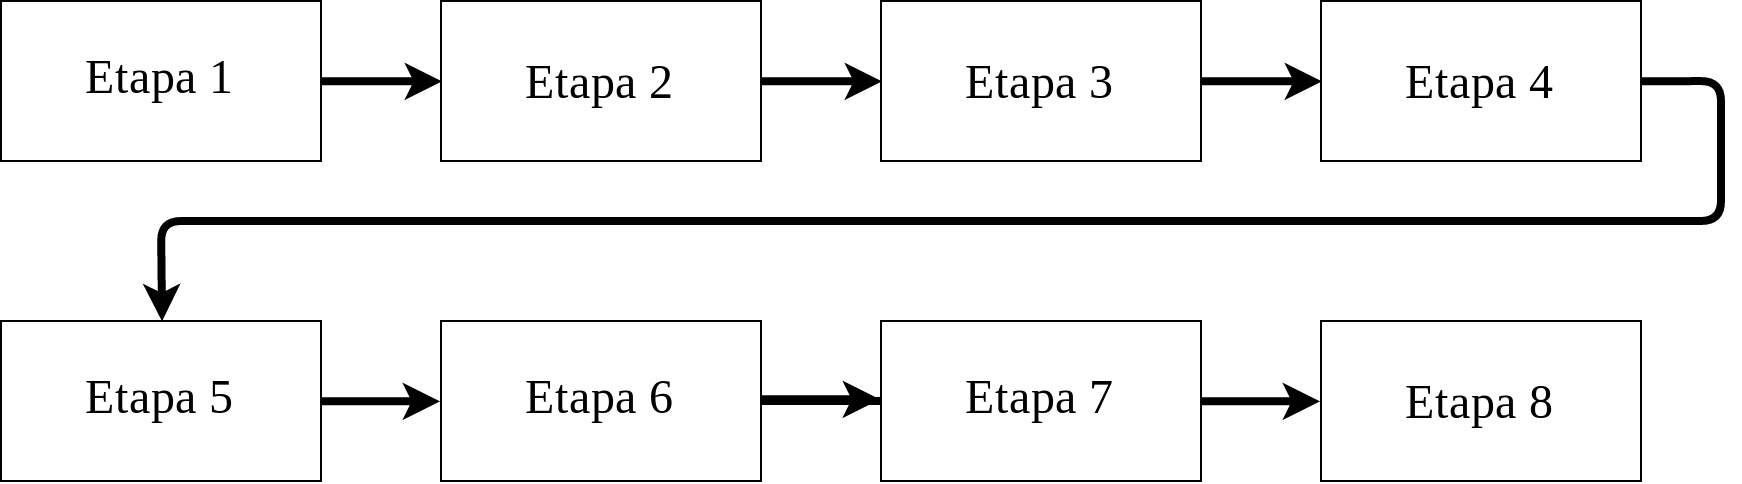
\includegraphics[width=\textwidth]{cap1_metodologia-etapas}
    \label{fig:cap1_metodologia-etapas}
    
    \footnotesize{Fonte: Autor}
\end{figure}

A seguir, a sequência de etapas demonstradas anteriormente são especificadas em detalhes.

\begin{itemize}\parskip -1pt
    \item Etapa 1: Análise e definição do escopo do trabalho.
	\item Etapa 2: Levantamento bibliográfico a cerca de Internet das Coisas e Sistemas de Recomendação;
	\item Etapa 3: Elaborar e desenvolver um projeto de leitura e monitoramento dos produtos contidos na geladeira.
	\item Etapa 4: Implementar um sistema de análise das interações e recomendação de serviços.
	\item Etapa 5: Desenvolvimento de um protótipo funcional que integre as Etapas 3 e 4.
	\item Etapa 6: Criação de um cenário de testes para avaliar o protótipo.
	\item Etapa 7: Avaliação e discussão dos resultados obtidos no cenário proposto.
	\item Etapa 8: Escrita do Trabalho de Conclusão de Curso.
\end{itemize}



% Colocar uma figura do fluxo
% Contextualizar para caracterizar
% O que vai usar 
% Teste
% Dizer como vai avaliar
% TODO: Descrição das etapas

\section{Organização do trabalho} % Não é necessário, no TCC 1

Este trabalho é divido em seis capítulos. O \textbf{Capítulo 1} apresentada uma introdução do estado da arte das áreas envolvidas bem como a problemática do trabalho e os objetivos gerais e específicos.

O \textbf{Capítulo \ref{cap:internet_of_things}} trata da Internet das Coisas, no qual é feita uma revisão da arquitetura para organização dos diversos componentes, das tecnologias existentes que possibilitam o desenvolvimento de novos dispositivos e, por fim, uma descrição sobre alguns dos ambientes nos quais a Internet das Coisas será incorporada nos próximos anos.

O \textbf{Capítulo \ref{cap:sistemas_de_recomendacao}} é sobre Sistemas de Recomendação

O \textbf{Capítulo 4} é sobre o Sistema Proposto

O \textbf{Capítulo 5} é sobre o cronograma para a displina de TCC II.

% O capítulo 5 é sobre a Avaliação do Sistema Proposto
% %	- Descrever um cenário
% %	- Avaliar e discutir o cenário a partir do sistema proposto
	
% O capítulo 6 é sobre Considerações Finais

% TODO: criar o arquivo para o organograma